\begin{example}[Three Nested While II]
    \label{ex:threeNestedWhileII}
    %
    $N < m < n$\\
    %
    % \[
    % %
    % \begin{array}{l}
    %     \kw{threeNestedWhileII}(k, m, N) \triangleq \\
    %     \clabel{ \assign{i}{0} }^{0} ; \\
    %         \ewhile ~ \clabel{i < k}^{1} ~ \edo ~ \\
    %         \qquad \Big(
    %          \highlight{\clabel{\assign{j}{i}}^{4}} ;\\
    %          \qquad \ewhile ~ \clabel{j > 0}^{5} ~ \edo ~ \\
    %          \qquad \qquad \Big(
    %           \clabel{\assign{j}{j-1}}^{6};
    %           \highlight{\clabel{\assign{w}{j}}^{6}};\\
    %           \qquad \qquad \ewhile ~ \clabel{w < N}^{5} ~ \edo ~
    %           \Big(
    %             \clabel{\assign{w}{w + 1}}^{6}
    %               \Big); \\
    %               \qquad \qquad \clabel{\assign{i}{w}}^{3}
    %               \Big); \\
    %               \qquad \clabel{\assign{i}{i+1}}^{3}
    %           \Big)
    %     \end{array}
    % \]
    {\small
  \begin{figure}
  \centering
  \begin{subfigure}{.4\textwidth}
    \begin{centering}
    {\small
    $
    \begin{array}{l}
        \kw{threeNestedWhileII}(k, m, N) \triangleq \\
        \clabel{ \assign{i}{0} }^{0} ; \\
            \ewhile ~ \clabel{i < k}^{1} ~ \edo ~ \\
            \qquad \Big(
             \highlight{\clabel{\assign{j}{i}}^{4}} ;\\
             \qquad \ewhile ~ \clabel{j > 0}^{5} ~ \edo ~ \\
             \qquad \qquad \Big(
              \clabel{\assign{j}{j-1}}^{6};
              \highlight{\clabel{\assign{w}{j}}^{6}};\\
              \qquad \qquad \ewhile ~ \clabel{w < N}^{5} ~ \edo ~
              \Big(
                \clabel{\assign{w}{w + 1}}^{6}
                  \Big); \\
                  \qquad \qquad \clabel{\assign{i}{w}}^{3}
                  \Big); \\
                  \qquad \clabel{\assign{i}{i+1}}^{3}
              \Big)
      \end{array}
    $
    }
    \caption{}
    \end{centering}
    \end{subfigure}
  \begin{subfigure}{.5\textwidth}
    \begin{centering}
  %   \todo{abstract-cfg for two round}
  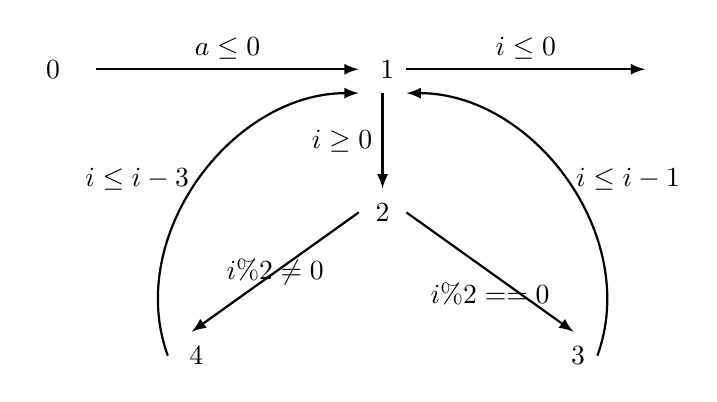
\begin{tikzpicture}[scale=\textwidth/20cm,samples=200]
  \draw[] (-7, 10) circle (0pt) node{{ $0$}};
  \draw[] (0, 10) circle (0pt) node{{ $1$}};
  \draw[] (0, 7) circle (0pt) node{\textbf{$2$}};
  \draw[] (4, 4) circle (0pt) node{{ $3$}};
  % \draw[] (0, 1) circle (0pt) node{{ $4$}};
  \draw[] (-4, 4) circle (0pt) node{{ $4$}};
  % Counter Variables
  \draw[] (6, 10) circle (0pt) node {\textbf{$\lex$}};
  % \draw[] (6, 4) circle (0pt) node {{ $ex$}};
  %
  % Control Flow Edges:
  \draw[ thick, -latex] (-6, 10)  -- node [above] {$a \leq 0$}(-0.5, 10);
  \draw[ thick, -latex] (0, 9.5)  -- node [left] {$i \geq 0$} (0, 7.5) ;
  \draw[ thick, -latex] (0.5, 7)  -- node [below] {$ i \% 2 == 0 $}  (4, 4.5);
  \draw[ thick, -latex] (-4.5, 4)  to  [out=110,in=180]  node [left] {$i \leq i - 3$ }(-0.5, 9.5);
  \draw[ thick, -latex] (4.5, 4)  to  [out=70,in=0]   node [right] {$i \leq i - 1$ }(0.5, 9.5);
  \draw[ thick, -latex]  (-0.5, 7) -- node  {$i \% 2 \neq 0$}  (-4, 4.5) ;
  \draw[ thick, -latex] (0.5, 10)  -- node [above] {$i \leq 0$}  (5.5, 10);
  % \draw[ thick, -latex] (6, 6.5)  -- node [right] {$\top$} (6, 4.5) ;
  \end{tikzpicture}
  \caption{}
    \end{centering}
    \end{subfigure}
  \caption{
  (a) The Simple While Loop Example with Two Paths
    (b) The Abstract Execution Control Flow Graph}
      \label{fig:whileOdd}
  \end{figure}
  }
\end{example}

\begin{enumerate}
    \item Step 1: Abstract Transition Graph:

\item Step 2: Path Insensitive Transition Bound Computation

\item Step 3: Program Rephrase through Path Collection on Abstract CFG
\\
$\tpath_0 = (0 \to 1)$
\\
$\tpath_1 = (1 \to 2),  (2 \to 3)$
\\
$\tpath_2 = (3 \to 4), (4 \to 5), (5 \to 6)$
\\
$\tpath_3 = (6 \to 7), (7 \to 6)$
\\
$\tpath_4 = (6 \to 8), (8 \to 3)$
\\
$\tpath_5 = (3 \to 9), (9 \to 1)$
\\
$\tpath_6 = (1 \to \lex)$
\\
Rephrased Program
\[
\tpath_0 ; LOOP1: \rprepeat(\tpath_1; LOOP2: \rprepeat(\tpath_2; LOOP3 : \rprepeat(\tpath_3); \tpath_4); \tpath_5); \tpath_6
\]
\item Step 4: While Loop Refinement:
\[
\tpath_0 ; LOOP1: \rprepeat(\tpath_1; LOOP2: \rprepeat(\tpath_2; LOOP3 : \rprepeat(\tpath_3); \tpath_4); \tpath_5); \tpath_6
\]
\item Step 5: Outside-In Algorithm
\\
$LB(\tpath_0) = 1$
\\
$LB(LOOP3 : \rprepeat(\tpath_3)) = N $
\\
$LB(LOOP2: \rprepeat(\tpath_2; \cdots)) = m $
\\
$LB(LOOP1: \rprepeat(\tpath_1; \cdots)) = n - N $
\\
\item Step 6: Inside-Out Algorithm
\begin{itemize}
    \item \textbf{Repeat Chain Set}
    \\
    $rp\mathcal{C}(LOOP1, \tpath_1) = \{\rprepeat(\tpath_1; \cdots)\}$ \\
    $rp\mathcal{C}(LOOP1, \tpath_5) = \{\rprepeat(\tpath_1; \cdots)\}$ \\
    $rp\mathcal{C}(LOOP2, \tpath_2) = \{\rprepeat(\tpath_2; \cdots)\}$ \\
    $rp\mathcal{C}(LOOP2, \tpath_4) = \{\rprepeat(\tpath_2; \cdots)\}$ \\
    $rp\mathcal{C}(LOOP3, \tpath_3) = \{\rprepeat(\tpath_3)\}$ \\
    $rp\mathcal{C}(_, \_) = \emptyset$ 
    % \\
    \item \textbf{{Local Repeat Chain Bound} for Every Transition Path $\tpath$ on its Repeat Chain}
    \\
    $rpLB(LOOP1, \tpath_1) = n - N$ \\
    $rpLB(LOOP1, \tpath_5) = n - N$ \\
    $rpLB(LOOP2, \tpath_2) = m$ \\
    $rpLB(LOOP2, \tpath_4) = m$ \\
    $rpLB(LOOP3, \tpath_3) = N$ \\
    $rpLB(_, \_) = \bot $ 
    %
    \item \textbf{Loop Chain Set}
    \\
    $lp\mathcal{C}(\tpath_1) = \{LOOP1\to \tpath_1\}$ \\
    $lp\mathcal{C}(\tpath_5) = \{LOOP1\to \tpath_5\}$ \\
    $lp\mathcal{C}(\tpath_2) = \{LOOP1 \to LOOP2 \to \tpath_2\}$ \\
    $lp\mathcal{C}(\tpath_4) = \{LOOP1 \to LOOP2 \to \tpath_4\}$ \\
    $lp\mathcal{C}(\tpath_3) = \{LOOP1 \to LOOP2 \to LOOP3 \to \tpath_3\}$ \\
    $lp\mathcal{C}(\tpath_0) = \{\tpath_0\}$ \\
    $lp\mathcal{C}(\tpath_6) = \{\tpath_6\}$ 
    \item \textbf{Nested Loop Bound for Every Transition Path $\tpath$ on its Loop Chain}
    \\
    $rpLB(LOOP1, \tpath_1) = n - N$ \\
    $rpLB(LOOP1, \tpath_5) = n - N$ \\
    $rpLB(LOOP1, \tpath_2) = m - N$;  $rpLB(LOOP2, \tpath_2) = m$; \\
    $rpLB(LOOP1, \tpath_4) = m - N$; $rpLB(LOOP2, \tpath_4) = m$ \\
    $rpLB(LOOP1, \tpath_3) = 1$; $rpLB(LOOP2, \tpath_3) = N$; $rpLB(LOOP3, \tpath_3) = N$ \\
    $rpLB(_, \_) = \bot $ 
    \item \textbf{Path Sensitive Reachability Bound For Every Transition Path $\tpath$ }
    \\
    $psRB(\tpath_1) = n - N$ \\
    $psRB(\tpath_5) = n - N$ \\
    \highlight{    
    $psRB(\tpath_2) = (m - N) \times m$ \\
    $psRB(\tpath_4) = (m - N) \times m$ \\}
    $psRB(\tpath_3) = N^2$ \\
    $psRB(\tpath_0) = 1$ \\
    $psRB(\tpath_6) = 1$ 
\end{itemize}
\item Step 7: Path Sensitive Reachability Bound Computation for Every Location
\\
$psRB(\{0, 1\}) = 1$ \\
$psRB(\{2, 3\}) = n - N$ \\
\highlight{
$psRB(\{4, 5, 6\}) = (m - N) \times m$ \\
$psRB(\{7, 6\}) = N^2$ \\
$psRB(\{8, 3\}) = (m - N) \times m$ \\
}
$psRB(\{9, 1\}) = n - N$ \\
$psRB(\{\lex\}) = 1$ 
\end{enumerate}